% !TeX document-id = {c68ea1ac-ebac-4541-a297-17005c6d2297}
% !TeX encoding = UTF-8
% !TeX spellcheck = en_US
% !TeX TS-program = pdflatex
% !TeX TXS-program:bibliography = biber -l zh__pinyin --output-safechars %

\documentclass[10pt]{article}

% to be `\input` in subfolders,
% ... therefore the path should be relative to subfolders.

\usepackage{iftex}
\ifPDFTeX
\else
	\usepackage[UTF8
		,heading=false
		,scheme=plain % English Document
	]{ctex}
\fi
%\ctexset{autoindent=true}
%\usepackage{indentfirst}
\setlength{\parindent}{0pt}

\input{../.modules/basics/macros.tex}
\input{../.modules/preamble_base.tex}
%\input{../.modules/preamble_notes.tex}
\input{../.modules/basics/biblatex.tex}


%Misc
%	\usepackage{lilyglyphs}
%	\newcommand{\indicator}{$\text{\clefG}$}
%	\newcommand{\indicatorInline}{$\text{\clefGInline}$}

\usepackage{titling}

\hypersetup{%
	colorlinks=true
	,linkcolor=DarkBlue
	,urlcolor=purple
	,linktoc=all
}


% Settings
\counterwithout{equation}{section}
\mathtoolsset{showonlyrefs=false}
%\DeclareTextFontCommand{\textbf}{\sffamily}

% Spacing
\usepackage[
	papersize={32cm,40cm},
	hmargin=1.5cm,
	vmargin={1.5cm,1.7cm}
]{geometry}
\geometry{footnotesep=2\baselineskip} % pre footnote split
\setlength{\parskip}{.5\baselineskip}
\renewcommand{\baselinestretch}{1.15}

\usepackage{ragged2e}

\usepackage{multicol}
\setlength{\columnsep}{2em}
\usepackage{enumitem}


%% List
	\setlist*{
%		noitemsep,
%		listparindent=\parindent
%		,labelindent=\parindent
%		parsep=\parskip
		nosep,
		parsep=\parskip,
		leftmargin=1.5em
	}


\usepackage{tikz}
\usepackage{caption}
%\usepackage{snapshot}

\renewenvironment{frame}[1]%
	{\section*{#1}}%
	{}

\newcommand{\citations}[1]{{\footnotesize#1\par}}
\newcommand{\reality}{reality\textsuperscript{TM}}

%\subtitle{An extended AdS\,/\,\TTbar duality \textit{(beyond infinity)}}


\newcommand{\veccol}[1]{\pqty{
	\begin{smallmatrix}
		#1
	\end{smallmatrix}
}}

\addbibresource{glueon-beamer.bib}
%\usepackage{cprotect}

\usepackage{cancel}
\newcommand{\slot}{{\,\bullet}}

\usepackage{xspace}
\newcommand{\TTbar}{\texorpdfstring{\ensuremath{T\bar{T}}}{TTbar}\xspace}

\newcommand{\jokeInfinity}{
	\includegraphics[height=.2\linewidth]{img/smbc-cantor-cropped.png}
\\[-.5ex]
	{\footnotesize\url{https://smbc-comics.com/comic/cantor}}
}

\setlength{\droptitle}{-3.25\baselineskip}
\pretitle{\LARGE\bfseries\noindent}
\title{Glue-on AdS holography for $T\bar T$-deformed CFTs}
\posttitle{\ \,\normalsize\textsl{JHEP 06 (2023) 117}}

\preauthor{\par\large\noindent}
\author{Wen-Xin Lai \textkai{赖文昕}}
\postauthor{, \textit{\normalsize with}
	Luis Apolo,
	Peng-Xiang Hao \textkai{郝鹏翔}
	and Wei Song \textkai{宋伟}
	\ \arxiv{2303.04836}
	\par%\vspace{.5\baselineskip}
	\vspace{-.6\baselineskip}
	\noindent\rule{.66\linewidth}{1pt}\par
	\vspace{-.1\baselineskip}
%	\vspace{.3\baselineskip}
}

\predate{\noindent\sffamily\,%
	Yau Mathematical Sciences Center YMSC, Tsinghua
	---
}
\date{July 2023}
\postdate{
	@ ICBS @ BIMSA
	\vspace{.5\baselineskip}
}

\pagestyle{empty}

\begin{document}

\maketitle
\thispagestyle{empty}


\begin{multicols}{3}

\noindent%
\textbf{Abstract:}
\TTbar-deformed CFTs with $\mu < 0$ have been proposed by \textcite{McGough:2016lol} to be holographically dual to Einstein gravity with a finite \mbox{Dirichlet} cutoff.

In this work we put forward a holographic proposal for \TTbar-deformed CFTs with $\mu > 0$, in which case the bulk dual geometry is constructed by gluing-on a patch of $\mrm{AdS}_3$ to the original spacetime. We provide various evidence for this extended holography, now valid for $\mu \in \mbb{R}$.

\vspace{.8\baselineskip}
\hrule
\vspace{.3\baselineskip}

We start from \textbf{pure Einstein gravity} without matter in $\mrm{AdS}_3$; the Einstein equations are solved by the metric:
\begin{equation}
\hspace{-2em}
\begin{aligned}
	ds^2
	&= \ell^2 \bigg( \frac{d\rho^2}{4 \rho^2} + \frac{ \big( du + \rho \, \mathcal {\bar L}(v)\, dv \big) \big( dv + \rho \, \mathcal L(u)\, du \big) }{\rho} \bigg)\\
	&= n_\mu n_\nu dx^\mu dx^\nu + \frac{1}{\zeta} \gamma_{ij}dx^i dx^j,\quad
\frac{1}{\zeta} \equiv \ell^{-2} g_{\varphi\varphi} \equiv r^2
\end{aligned}
\label{fggauge}
\end{equation}
The radial coordinate: $\rho \approx r^{-2} \equiv \zeta$,
where $r$ is the ``proper radius''; $\mathcal L(u)$ and $\bar{\mathcal L}(v)$ are arbitrary periodic functions.

\noindent%
The geometry is foliated by constant $\zeta$ surfaces ${\mathcal N}_\zeta$. 
\\
The asymptotic boundary $\mcal{N}_0$ is at $\zeta \to 0$, with coordinates: $x^{i} \sim \varphi, t$, while $u,v = \varphi \pm t$.

\noindent\citations{%
\textcite{Fefferman:2007rka}\\
\textcite{Banados:1992wn}\\
\textcite{Banados:1998gg}
}
\vspace{-.5\baselineskip}
\subsection*{Foundations: $\mrm{AdS}_3/\mrm{CFT}_2$ holography}
\vspace{-.5\baselineskip}
\begin{align*}
%\hspace{-1em}
	\textrm{\textit{asympt.}~$\mrm{AdS}_3$ Gravity}
	&\ \equiv\ 
	\textrm{Large $N$ $\mrm{CFT}_2$ at $\mcal{N}_0$}
\end{align*}

\citations{\noindent%
	\textcite{Maldacena:1997re}\\
	\textcite{Aharony:1999ti} \textit{et al}
}
%\begin{center}
%	\includegraphics[width=.7\linewidth]{img/ads-cft.png}\\[.5ex]
%	\scriptsize\ Image courtesy: \textcite{AldegundePWSep22}
%\end{center}

%\begin{itemize}

%\item Universal / ubiquitous:
%
%\begin{itemize}
%	\item Model agnostic: $\mrm{AdS}_5\times S^5$, $\mrm{AdS}_3\times S^3 \times T^4$, symmetric orbifolds, minimal models, ``monsters'', ... \textit{\small Maldacena, Witten, GKP, ABJM, Gaberdiel, and many many more}
%	
%\end{itemize}

%\end{itemize}

\begin{itemize}

\item Define \textbf{``\,$\TTbar$\,'' deformation} as the flow of action:
\begin{equation}
	\partial_{\sidenote{\mu}} I = {8 \pi} \int d^2x \, T\bar T_{(\sidenote{\mu})} = {\pi} \int d^2x\,\big( T^{ij}T_{ij}- (T^i_i)^2 \big)_{(\sidenote{\mu})}
	\label{TTbardef}
\end{equation}
where $x, \bar{x} = \varphi' \pm t'$.
We shall start from $\mrm{CFT}_2$ such that $T\bar{T}_{(\mu = 0)} = T_{xx} T_{\bar{x}\bar{x}}$, but note that the deformation is \textit{irrelevant}: conformal symmetry will be broken for $\mu \ne 0$.

\item \textbf{Solvable:} the deformed spectrum of $\hat{H}(\mu)$ and $\hat{J}(\mu)$ on a cylinder of radius $R$ is a simple function:
\begin{equation}
\hspace{-2em}
\begin{gathered}
	E(\mu) = - \frac{R }{ 2\mu } \bigg(1-\sqrt{1 + \frac{4\mu}{R} E(0) + \frac{4\mu^2}{R^4} J(0)^2 }
	\,\bigg), \\ J(\mu)=J(0) \\[-1.5ex]
\end{gathered} \label{ttbarspectrum}
\end{equation}
of the undeformed spectrum $E(0)$, $J(0)$,
under reasonable assumptions (e.g.~translation invariance). 

\citations{
\textcite{Zamolodchikov:2004ce}\\
\textcite{Dubovsky:2012wk}\\
\textcite{Dubovsky:2013ira}\\
\textcite{Smirnov:2016lqw}\\
\textcite{Cavaglia:2016oda}\\
\textcite{Dubovsky:2017cnj} \textit{et al}
}

\vspace{-.5\baselineskip}

\end{itemize}

\subsection*{Cutoff $\mrm{AdS}_3$ duality:\texstringonly{\\} Holography within a finite Dirichlet wall}

\citations{
\textcite{McGough:2016lol}\\
\textcite{Kraus:2018xrn} \textit{et al}
}

\textbf{Dictionary:} the \TTbar deformed theory lives on $\mcal{N}_{\zeta_c}$ with metric $\gamma_{ij}$.
Location (radius) of the cutoff surface gets mapped to the deformation parameter $\mu$:
\begin{equation}
	\zeta_c = - \frac{c \mu}{3\ell^2}
	\label{dictionary}
\end{equation}
\TTbar flow is recast geometrically as the $i,j$ components of the Einstein equations. This is a ``non-AdS'' / non-CFT duality.

\noindent%
\textit{A step towards quantum gravity in \reality!}

\columnbreak

\vspace*{-4\baselineskip}
\begin{center}
	\hspace{.1\linewidth}
	\includegraphics[width=.4\linewidth]{img/cutoff-ads.jpg}
	
	\vspace{-.5\baselineskip}\small
	Cutoff $\mrm{AdS}_3$\,/\,\TTbar-deformed $\mrm{CFT}_2$

	\vspace{-.2\baselineskip}
	\scriptsize\ Image courtesy: \textcite{AldegundePWSep22}
\end{center}


\begin{itemize}

\item[] \textbf{Caveat:} the duality only admits $\zeta_c > 0$ so $\mu < 0$.\\
But \TTbar itself admits $\mu > 0$ with cool properties.

\citations{The related proposal of \textcite{Guica:2019nzm}\\
admits both signs of $\mu$.}

\textit{What is the other side of the duality?}

\end{itemize}

\vspace{-\baselineskip}

\section*{\textbf{Proposal:}\texstringonly{\\}Glue-on $\mrm{AdS}_3$ -- beyond the infinity}
\label{se:glueonproposal}

\parbox{\linewidth}{
\vspace{-\baselineskip}
\begin{equation*}
\hspace{-.8em}
	\textrm{Cutoff / \textit{glue-on} $\mrm{AdS}_{d+1}$ Gravity}
	\ \equiv\ %
	\textrm{\TTbar deformed $\mrm{CFT}_{d}$ at $\mcal{N}_{\zeta_c}$}
\end{equation*}
\begin{center}
	\vspace{-.8\baselineskip}%
	\centering
	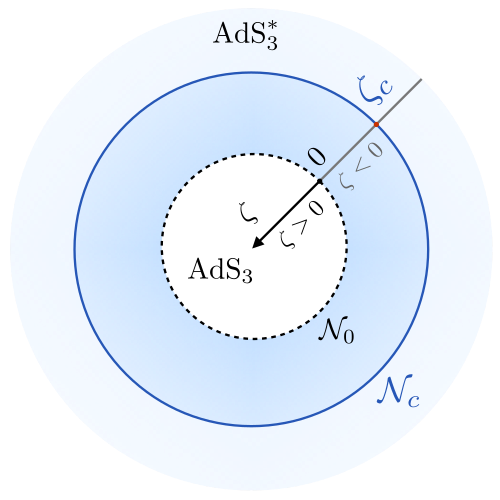
\includegraphics[width=.6\linewidth]{img/diagram.pdf}
	
	\vspace{-.5\baselineskip}
	\scriptsize\ Top-down view of a constant $t$ slice
\end{center}
%\vspace{-\baselineskip}
}

\begin{itemize}

\item \textbf{Analytic continuation:} metric \eqref{fggauge} has a simple pole, thus admits well-defined analytic continuation:
%\begin{equation}
%	\rho,\ \zeta,\ \mu\ \in\ \mbb{R}
%\end{equation}
\begin{equation}
	\frac{1}{\zeta} \equiv \ell^{-2} g_{\varphi\varphi} \in \mbb{R},
\ \quad
	\zeta_c = - \frac{c \mu}{3\ell^2} \in \mbb{R}
\end{equation}
What are we doing other than copy-pasting?
	\begin{itemize}
	\item Physical quantities diverge as $\zeta \to 0$.
	A prescription is required to ``renormalize'' the divergences.
	
	\item Treatment for the singularity at $\zeta\to 0^\pm$: introduce $\mathcal N_{\zeta={\pm\epsilon}}$ and glue them together (``\textbf{glue-on}'');
		exclude the $-\epsilon < \zeta < \epsilon$ region until finally sending $\epsilon \to 0$. 
%	\item We formally denote the boundary surface by the limit $\mathcal N_{0}=\mathcal N_{0^+}=\mathcal N_{0^-}$, though we need to keep track of the asymptotic cutoff $\epsilon$ in actual computations.
	\end{itemize}
	
\item \textbf{Extending the flow:} matching energy momentum (Brown-York) \& the \TTbar flow equations:
	\begin{equation}
	\begin{gathered}
		T_{ij}= \frac{\sigma_{\zeta_c}}{8\pi G} \Big( K_{ij} -  K \gamma_{ij} + \frac{1}{\ell |\zeta_c|}\gamma_{ij}\Big), \\ \sigma_{\zeta_c} = \tfrac{\abs{\zeta_c}}{\zeta_c} = \pm 1,\quad
		\gamma_{ij} = \zeta_c h_{ij}, \\[-1ex]
	\end{gathered}	\label{BYtensor}
	\end{equation}
	where $h_{ij}$ is the induced metric. 
	
	The field theory metric $\gamma_{ij}$ is always positive-definite, while $h_{ij}$ becomes negative-definite for the glue-on region $\rho,\zeta < 0$.
	This discrepancy is the origin of the $\abs{\zeta_c}$.

%\end{itemize}
%
%\subsection*{\TTbar physics from the glue-on geometry}
%
%\begin{itemize}

\item Demanding a \textbf{non-singular extended geometry} reproduces bounds on the \TTbar deformed theory, e.g.
	\begin{equation}
		\zeta_c \ge -1 \quad \Leftrightarrow \quad\mu\le \frac{ 3\ell^2 }{c} \label{reality}
	\end{equation}
	This is a Killing horizon in the glue-on region of the \mbox{extended} geometry;
	$(\det g_{\mu\nu})_{\,\zeta = -1} = 0$.

\item \textbf{Spectrum from the extended geometry:} they are \mbox{conserved} charges of the Killing symmetries, and can be computed with the \textit{covariant formalism}.

\citations{
	\textsl{\citeauthor{Iyer:1994ys,Barnich:2001jy}} et al\\
	With \TTbar: \textcite{Kraus:2021cwf}
}\vspace{-1.5\baselineskip}
	\begin{align*}
		\delta E(\mu) &\equiv  \ell^{-1} \delta \mathcal Q_{\pd_{t'}}, \quad \delta J(\mu) \equiv  \delta \mathcal Q_{\pd_{\varphi'}}.
	\end{align*}
	This reproduces $E(\mu)$, $J(\mu)$ with $\mu \in\mbb{R}$ in \eqref{ttbarspectrum}.

\columnbreak

\vspace*{-8\baselineskip}
%\item The covariant charges (variation):

	\item To match the bulk \& boundary symmetries at $\mcal{N}_{\zeta_c}$, we choose the appropriate coordinates $(t',\varphi')$, such that
	\begin{equation}
		ds^2_c = \ell^2 ( -dt'^2 + d\varphi'^2) , \qquad \varphi' \sim \varphi' + 2\pi.\label{cutoffmetric}
	\end{equation}
This is realized by:
	\begin{align*}
		dt' &= \sqrt{ \big(1 - \zeta_c (T_u+T_v)^2 \big) \big(1 - \zeta_c (T_u-T_v)^2 \big) } \, dt,  \\
		 d\varphi' &= d\varphi + \zeta_c \big( T_u^2 - T_v^2 \big)\,dt.
	\end{align*}

\item The above \textbf{\textit{state-dependent} map of \mbox{coordinates}} leads to the correct charges, the modified signal propagation speed $v'_{\pm} \equiv \pm {d\varphi'}/{dt'}$, and the \TTbar \textbf{thermodynamics} when Wick rotated. In particular,
	\begin{equation*}
	\hspace{-.5em} \mu > 0,\quad
		T_L(\mu)\,T_R(\mu) \le - \frac{1}{4\pi^2 \ell^2 \zeta_c} = \frac{3}{4\pi^2c\mu} = T_H(\mu)^2.
	\end{equation*}
	$T_{L,R}$ are temperatures associated with $u',v' = \varphi' \pm t'$.\\
	$T_H$ is the \textit{Hagedorn temperature}: exceeding $T_H$ leads to a complex entropy.

\begin{flushright}
\vspace{-.5\baselineskip}
\citations{
\textcite{Giveon:2017nie}\\
\textcite{Apolo:2019zai}
}
\vspace{-\baselineskip}
\end{flushright}

\end{itemize}

\subsection*{\TTbar partition functions from bulk actions} \label{se:partitionfunction}

\begin{itemize}
\item The \TTbar partition function is approximated by the bulk on-shell action of the dominant saddle:
	\begin{equation}
		Z_{T\bar T} (\mu) = \mathcal Z (\zeta_c) \approx  e^{-I(\zeta_c)}. \label{partition2}
	\end{equation}
$I(\zeta_c)$ \mbox{diverges} at $\zeta \to 0^\pm$. We apply a natural extension of \textit{holographic renormalization} to remove the divergence.
It includes the boundary action (with counterterms):
	\begin{align}
%		I_{\mcal{M}}(\zeta_1, \zeta_2) & \coloneqq - \frac{1}{16\pi G} \int_{\zeta_1}^{\zeta_2} d\zeta \int d^2 x \sqrt{g} \, (R + 2 \ell^{-2}),  %\label{bulkaction} \\
%	\\
		I_{\mathcal N_{\zeta}} & \coloneqq  - \frac{1}{8\pi G} \int_{\mathcal N_{\zeta}} d^2x \sqrt{h}\,h^{ij} K_{ij} \notag
	\\& \qquad + \frac{\sigma_\zeta}{8\pi G} \int_{\mathcal N_{\zeta}} d^2x \sqrt{h} \, \bigg(\ell^{-1} - \frac{\ell  \mathcal{R}[h]}{4} \log |\zeta| \bigg). \label{boundaryaction}
	\end{align}
	The lack of diff invariance of the $\log |\zeta|$ counterterm is known to be a reflection of the Weyl anomaly. 
	The \mbox{action} is consistent with the Brown-York stress \mbox{tensor} in \eqref{BYtensor}. 

	\hfill{\footnotesize \textcite{Henningson:1998gx} \textit{et al}}

The resulting $I = -\log \mcal{Z}$ satisfies the \TTbar flow \eqref{TTbardef}.\\
Furthermore, it agrees with the field theory analysis:

\item \textbf{Torus:} {modular invariance} \& sparseness of the ``light'' spectrum at large $c$ leads to the universal form :
	\begin{equation*}\small
	\hspace{-1.5em}
		\log   Z_{T\bar T}(\mu)  \approx \left\{ \begin{aligned}
		& {-\frac{1}{2}}\,(\beta_L + \beta_R)\, RE_{\text{vac}}(\mu),  &\beta_L \beta_R > 1, \\
		& {-2 \pi^2 \bigg(\frac{1}{\beta_L} + \frac{1}{\beta_R}\bigg)  RE_{\text{vac}}\bigg(\frac{4\pi^2}{\beta_L \beta_R} \mu \bigg)},  &\beta_L\beta_R < 1. %\\[2ex]
		 \end{aligned} \right. %\label{ZTTbar}
	\end{equation*}
	\citations{\noindent%
		\textcite{Datta:2018thy}\\
		\textcite{Apolo:2023aho}\\
		cf.~\textcite{Hartman:2014oaa}
%		\textcite{Apolo:2023aho}, \mbox{following \textcite{Datta:2018thy} and \textsl{\citeauthor{Hartman:2014oaa}}}
	}

\item \textbf{Sphere:} maximally symmetric,\\ \mbox{\footnotesize \textcite{Donnelly:2018bef}}
	\begin{equation}
%		\label{sphere:stresstensor}
		\langle T_{ij}\rangle = -\frac{1}{4\pi\mu} \bigg(1-\sqrt{1-\frac{c\mu}{3R^2}}\, \bigg)  \gamma_{ij}.
	\end{equation}
Then the trace relation \mbox{$
%	\begin{align*}
%\partial_\mu \log Z_{\TTbar}(\mu)&=8\pi \int d^2x\sqrt{\gamma}\, \langle T\bar{T} \rangle \\
(-R)\,\partial_R \log Z_{\TTbar}(\mu)=\int d^2x\sqrt{\gamma}\,\langle T^i_i \rangle
%	\end{align*}
$} along with the flow equation \eqref{TTbardef} 
admits the general \mbox{solution} with a $\mu$-\textit{independent} integration constant $a$:
	\begin{equation*}\small
	\hspace{-1.2em}
		\log Z_{\TTbar}(\mu, a) = \frac{c}{3} \log \bigg[\frac{R}{a}   \bigg(1+\sqrt{1-\frac{c \mu }{3  R^2}}\, \bigg) \bigg] - \frac{R^2}{\mu}  \sqrt{1-\frac{c \mu }{3 R^2}} + \frac{R^2}{\mu}. %\label{Zsol}
	\end{equation*}
	\cite{Donnelly:2018bef} is recovered with $a = \sqrt{c|\mu|/3}$ but one can also take $a = \epsilon$, thus decoupling the renormalization length scale $\epsilon$ with the deformation $\mu$. In general the space of deformed theories can be parametrized by independent $(\mu,a)$.

	The $\log$ counterterm in \eqref{boundaryaction} makes a crucial contribution to the on-shell action; it guarantees that the partition function is compatible with the $T\bar T$ differential equation, which is not the case for \cite{Donnelly:2018bef}.
	\begin{flushright}
		\vspace{-.6\baselineskip}
		\citations{
			\textcite{Caputa:2020lpa}\\
			\textcite{Li:2020zjb}
		}\vspace{-.8\baselineskip}
	\end{flushright}
	
	\item Following these results, we would like to understand the entanglement structure of \TTbar deformed theories with the help of bulk geometry in future studies.
	\begin{flushright}
		\vspace{-.5\baselineskip}
		\citations{
			\textcite{Lewkowycz:2019xse}
		}
	\end{flushright}
\end{itemize}

%\begin{center}
%	\includegraphics[width=.5\linewidth]{img/RT-AdS.pdf}
%	
%	\vspace{-.8\baselineskip}
%	RT surface for the extended $\mrm{AdS}_3$
%\end{center}
%
%\citations{
%\begin{itemize}[noitemsep]
%\item \textcite{He:2023xnb}
%\item \textcite{He:2023wko}
%\item \textcite{Tian:2023fgf}
%\end{itemize}
%}
%
%\renewcommand*{\bibfont}{\footnotesize}
%\printbibliography %%% should not specify heading

\end{multicols}

\end{document}
